\documentclass[titlepage]{article}
\usepackage[a4paper,includehead,includefoot,headheight=10pt,headsep=2mm,width=17cm,height=27cm,footskip=0.5cm]{geometry}
\usepackage{cmap}
\usepackage{hyperref}
\usepackage[T1]{fontenc}
\usepackage[utf8]{inputenc}
\usepackage[russian]{babel}
\usepackage{graphicx}
\usepackage{xcolor}
\usepackage{amssymb}
\usepackage{amsmath}
\usepackage{physics}
\usepackage{wrapfig}

\usepackage{pgfplots}
\pgfplotsset{width=7cm,compat=newest}

\usepackage{amsmath}
\DeclareMathOperator\arctanh{arctanh}

\usepackage{amsmath}
\DeclareMathOperator\arccosh{arccosh}

\usepackage{amsmath}
\DeclareMathOperator\const{const}

\begin{document}

\begin{abstract}
Курс ядерной физики СПБГУ 
\end{abstract}

\section{Введение}
Данный курс посвящён науке, занимающей изучением мельчайших объектов нашего мира --- атомных ядер. Данная наука охватывает самые разные временные и пространственные масштабы. Ядерные взаимодействия появились после нескольких секунд после рождения Вселенной. С их помощью описываются звёзды, нейтронные звёзды можно рассматривать как большое атомное ядро. 

\par
Ядерная физика~\----~не только ядерная бомба, она охватывает гораздо более широкую область человеческих знаний, это и криминалистика, энергетика, медицина, производство новых материалов и археология. 

\section{Состав атомных ядер. Радиоактивность}
Одно из главных достижений человечества~\----~постижение идеи атомизма, которая заключается в том, что всё из чего\--то состоит. Например, ядра состоят из нуклонов, нуклоны~\----~из протонов и нейтронов, протоны из кварков, кварки взаимодействуют с помощью глюонов и так далее.

\begin{wrapfigure}{R}{0.35\textwidth}
\centering
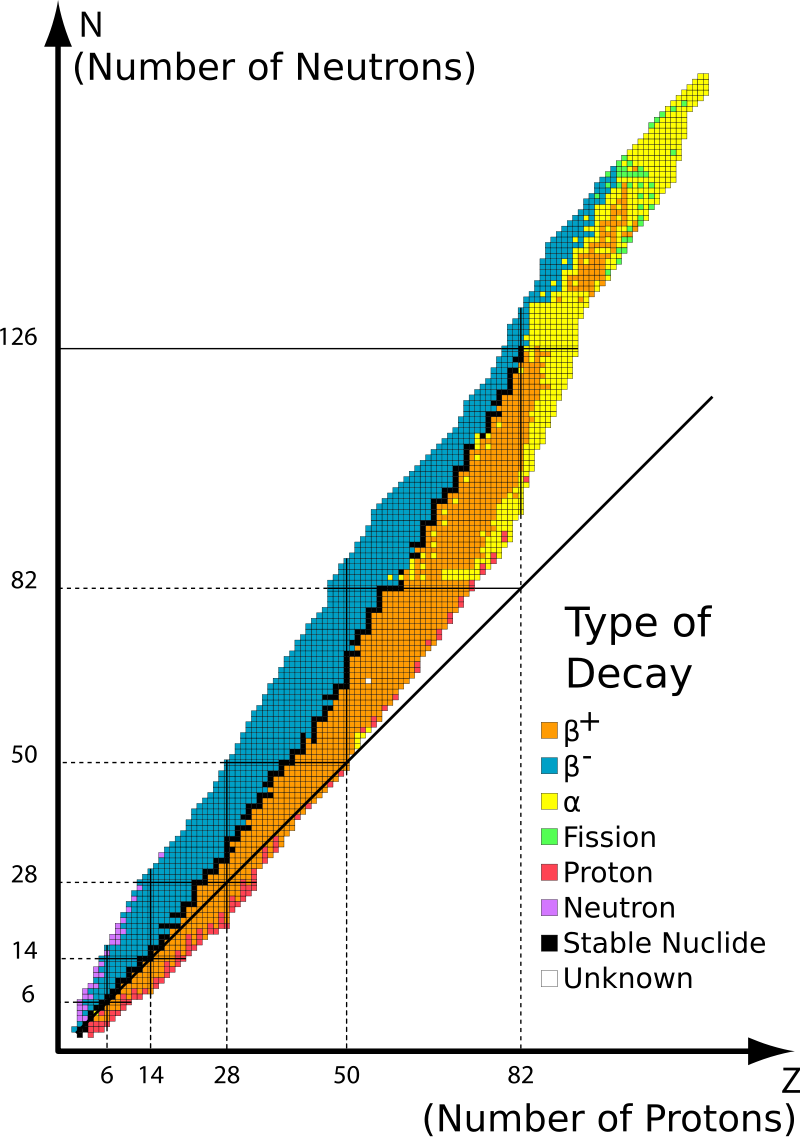
\includegraphics[width=0.3\textwidth]{1.png}
\caption{\label{1}Диаграмма $N \times Z$ радиоактивности}
\end{wrapfigure}

\subsection{Состав атомного ядра}
Атомное ядро есть квантово\--механическая система, поэтому состав атомных ядер определятся той энергией, которую мы рассматриваем, ибо при рассмотрении больших энергий возможен пробой вакуума (рождение электрон-позитронных пар), что приводит к неопределённости состава ядра.

\par
Пускай, под рассмотрением находятся малые энергии. Тогда можно сказать, что атомное ядро состоит из \emph{нуклонов}~\----~протонов и нейтронов. Атомное ядро обозначается элементом, центром которого является ядро. Важными характеристиками ядра являются \emph{массовое число} $A$~\----~число нуклонов в ядре, \emph{зарядовый номер элемента} $Z$~\----~число протонов в ядре и \emph{число нейтронов} $N$. Используется следующий вид обозначения атомного ядра:

\begin{equation}
 {}^{A}_{Z} El_N, \text{где } A = Z + N
\end{equation}

Выделяют следующие типы ядер:
\begin{enumerate}
 \item \emph{Изобары}~\----~ядра с одинаковым числом нуклонов:
 $
 A = \const
 $
 \item \emph{Изотопы}~\----~ядра с одинаковым зарядовым числом:
 $
 Z = \const
 $
 \item \emph{Изотоны}~\----~ядра с одинаковым числом нейтронов:
 $
 N = \const
 $
\end{enumerate}

\subsection{Радиоактивность}
На диаграммах $N \times Z$ все существующие ядра образуют узкую область на диагонали, в середине этой области имеет место быть так называемая \emph{полоса $\beta$\--стабильности}, состоящая из стабильных ядер, по мере удаления от этого островка стабильности время жизни ядер уменьшается и, в конце концов, они вообще перестают существовать. Иными словами, при удалении от полосы $\beta$\--стабильности увеличивается \emph{радиоактивность} ядер.

\subsection{Время жизни ядер}
Основной мерой радиоактивности ядер является время их жизни. \emph{Время жизни ядер} определяется \emph{законом радиоактивного распада}:
\begin{equation}\label{zrr}
 \dd N = -\lambda N \dd t
\end{equation}
Откуда незамедлительно получаем:
\begin{equation}\label{zrr1}
 N\qty(t) = N_0 \exp(-\lambda t)
\end{equation}
В формулах (\ref{zrr}) и (\ref{zrr1}) за $\lambda$ обозначена \emph{вероятность распада}, за $N$~\----~количество оставшихся ядер и за $t$~\----~время, прошедшее с момента, когда количество ядер было равно $N_0$.

\begin{wrapfigure}{R}{0.35\textwidth}
\centering
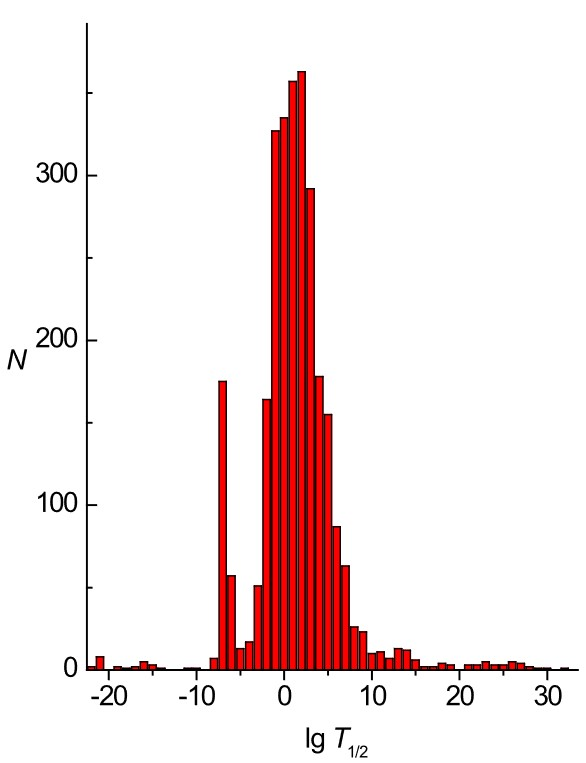
\includegraphics[width=0.3\textwidth]{2.jpg}
\caption{\label{2}Гистограмма периода полураспада ядер}
\end{wrapfigure}

\par
Вероятность распада определяет многие важные на практике характеристики ядра, например, такие, как количество ядер, распавшихся за время $t$:
\begin{equation}
 N_0 - N\qty(t) = N_0\qty(1-\exp(-\lambda t))
\end{equation}
Кроме того, вероятность распада определяет \emph{период полураспада} (период времени, за который успевает распасться половина от исходного количества ядер):
\begin{equation}
 T_{\tfrac{1}{2}} =  \dfrac{\ln{2}}{\lambda}
\end{equation}
На приведённой ниже гистограмме (\ref{2}) показано, что период полураспада ядер может принимать широкий спектр значений от $10^{-23}$ секунд до $10^{30}$ секунд.

\par
Наибольший интерес представляет середина этого набора нуклидов~\----~\emph{стабильные ядра}. На карте нуклидов (\ref{3}) можно видеть несколько сечений по $Z$, то есть несколько химических элементов, содержащие несколько стабильных изотопов (на карте им отвечают чёрные точки). В этом нет ничего удивительного, например, водород представлен двумя стабильными изотопами: протий ${}^1 H$ (просто протон) и дейтерий ${}^2 H$ (протон и нейтрон), кислород~\----~тремя и так далее.

\begin{figure}[htb]
 \centering
 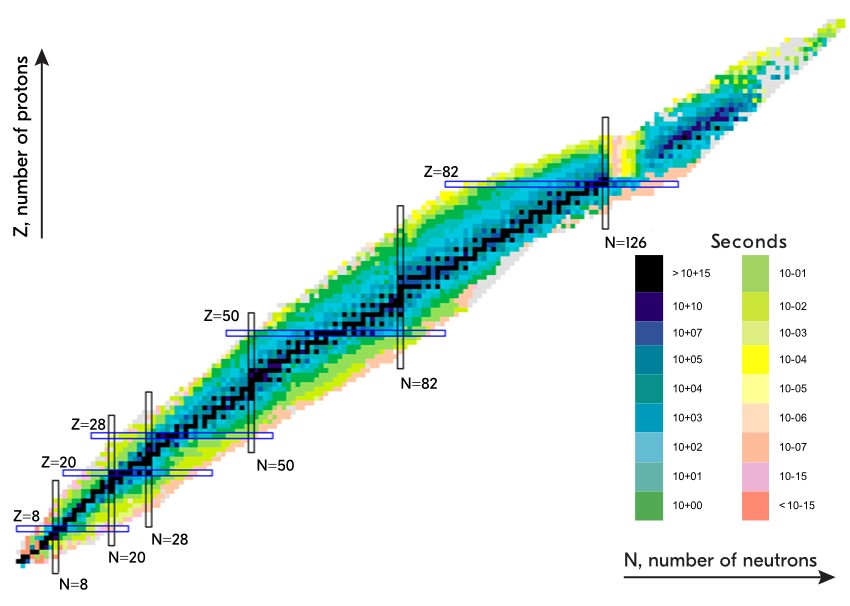
\includegraphics[width=110mm]{3.jpg}
 \caption{Карта нуклидов}
 \label{3}
\end{figure}
\end{document}
